\documentclass[a4paper,10pt]{article}

\usepackage[top=1cm,bottom=1cm,left=1.3cm,right=1.3cm]{geometry}
\usepackage{fontspec}
\setmainfont{TeX Gyre Pagella}
\usepackage{unicode-math}
\setmathfont{TeX Gyre Pagella Math}

\usepackage{tikz}
\usetikzlibrary{arrows.meta,calc,positioning,shapes.geometric}
\usepackage{microtype}

\pagestyle{empty}
\setlength{\parindent}{0pt}
\setlength{\parskip}{0.2em}

% Lyskjegle-kommando
% Argumentar: #1 = horisontal radius (cm), #2 = vertikal radius (cm)
\newcommand{\lyskjegle}[2]{%
  \begin{tikzpicture}[baseline=0pt,line width=0.3pt]
    \coordinate (T) at (0, #2);
    \coordinate (B) at (0, -#2);
    \coordinate (L) at (-#1, 0);
    \coordinate (R) at (#1, 0);
    \draw (T) -- (R) -- (B) -- (L) -- cycle;
    \draw[dashed,black!45,line width=0.2pt] (L) -- (R);
  \end{tikzpicture}%
}

% Samansett lyskjegle med tre indre diamantar
\newcommand{\lyskjeglesaman}[2]{%
  \begin{tikzpicture}[baseline=0pt,line width=0.3pt]
    \coordinate (T) at (0, #2);
    \coordinate (B) at (0, -#2);
    \coordinate (L) at (-#1, 0);
    \coordinate (R) at (#1, 0);
    \draw (T) -- (R) -- (B) -- (L) -- cycle;
    \draw[dashed,black!45,line width=0.2pt] (L) -- (R);
    % Tre indre diamantar
    \pgfmathsetmacro{\ir}{#1*0.25}
    \pgfmathsetmacro{\iv}{#2*0.25}
    \foreach \dx in {-0.5,0,0.5} {
      \pgfmathsetmacro{\cx}{\dx * #1 * 0.7}
      \draw[line width=0.22pt] (\cx, \iv) -- (\cx+\ir, 0) -- (\cx, -\iv) -- (\cx-\ir, 0) -- cycle;
      \draw[dashed,black!35,line width=0.15pt] (\cx-\ir, 0) -- (\cx+\ir, 0);
    }
  \end{tikzpicture}%
}

\begin{document}

\begin{center}
{\Large\scshape Skalahierarki}\hspace{0.6em}{\itshape Kognitive lyskjegler frå kvark til sivilisasjon}
\end{center}

\vspace{-0.4em}

\begin{center}
\rule{\textwidth}{0.3pt}
\end{center}

\vspace{0.1em}

{\small Kvar agent har si eiga lyskjegle. Diamantforma representerer tre parametrar samstundes: framtidshorisont (oppover), fortidshorisont (nedover), og romleg rekkjevidde (horisontal linje gjennom midten). Lyskjegla er isomorf på tvers av skalaer; berre parametrane endrar seg. Dei samansette lyskjeglene på dei tre øvste nivåa syner at multiagens er multiskalar: eit samfunn er bokstaveleg ei lyskjegle som inneheld lyskjegler.}

\vspace{0.1em}

\begin{center}
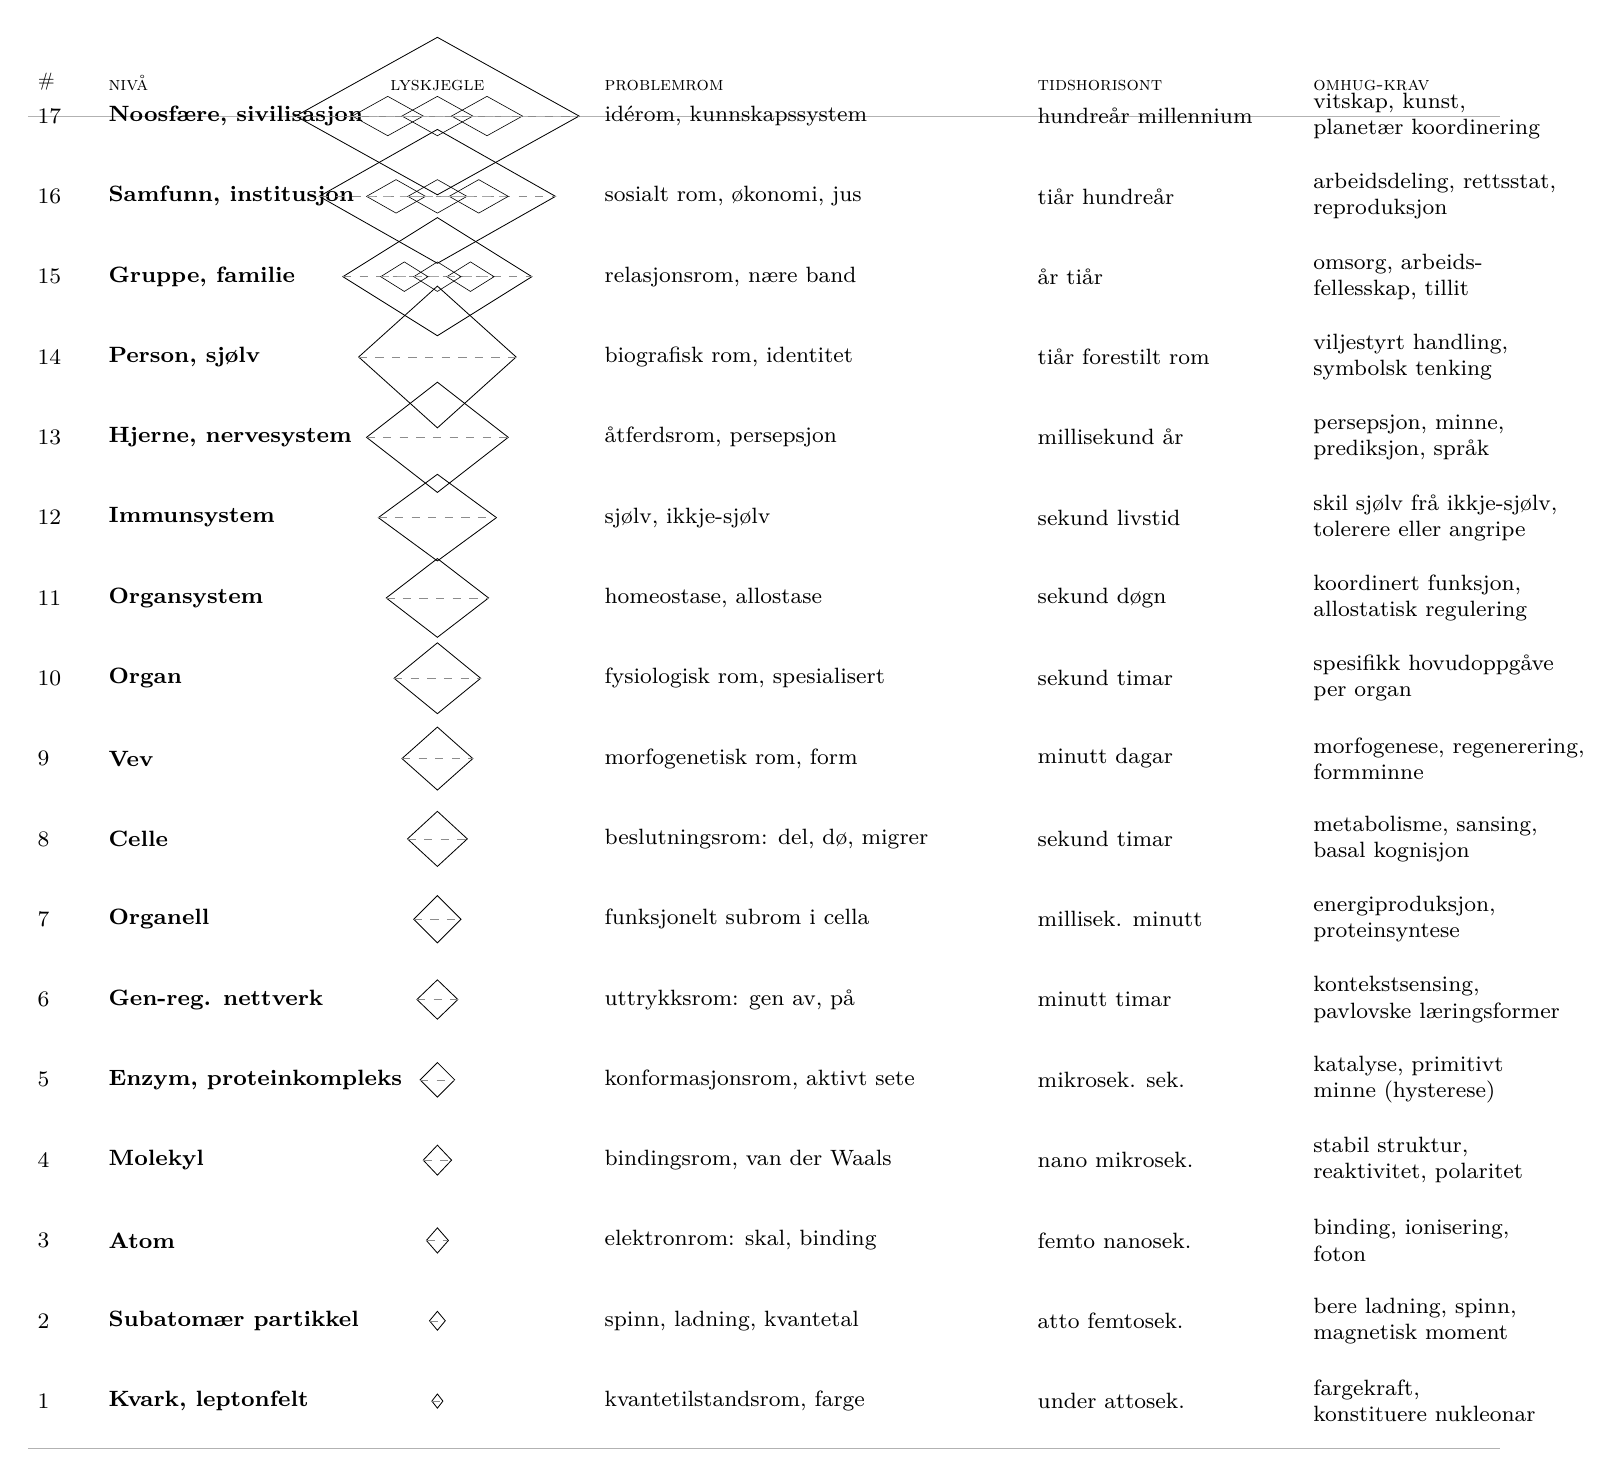
\begin{tikzpicture}[x=1cm,y=1cm,font=\footnotesize]

  % Header
  \node[anchor=south west,font=\scriptsize\scshape] at (-0.2, 0.2)  {\#};
  \node[anchor=south west,font=\scriptsize\scshape] at (0.7, 0.2)  {nivå};
  \node[anchor=south,font=\scriptsize\scshape]     at (5.0, 0.2)  {lyskjegle};
  \node[anchor=south west,font=\scriptsize\scshape] at (7.0, 0.2)  {problemrom};
  \node[anchor=south west,font=\scriptsize\scshape] at (12.5, 0.2) {tidshorisont};
  \node[anchor=south west,font=\scriptsize\scshape] at (16.0, 0.2) {omhug-krav};
  \draw[black!30,line width=0.2pt] (-0.2, 0) -- (18.5, 0);

  % Row function parameters:
  % \i = row index (0 = top, 16 = bottom)
  % We draw each row manually for precise control

  % y-steg per rad
  \def\rs{-1.02}

  % Level 17: Noosfære
  \node[anchor=west] at (-0.2, 0+0*\rs) {17};
  \node[anchor=west] at (0.7, 0+0*\rs) {\textbf{Noosfære, sivilisasjon}};
  \node at (5.0, 0+0*\rs) {\lyskjeglesaman{1.8}{1.0}};
  \node[anchor=west] at (7.0, 0+0*\rs) {idérom, kunnskapssystem};
  \node[anchor=west] at (12.5, 0+0*\rs) {hundreår  millennium};
  \node[anchor=west,align=left] at (16.0, 0+0*\rs) {vitskap, kunst,\\planetær koordinering};

  % Level 16: Samfunn
  \node[anchor=west] at (-0.2, 0+1*\rs) {16};
  \node[anchor=west] at (0.7, 0+1*\rs) {\textbf{Samfunn, institusjon}};
  \node at (5.0, 0+1*\rs) {\lyskjeglesaman{1.5}{0.85}};
  \node[anchor=west] at (7.0, 0+1*\rs) {sosialt rom, økonomi, jus};
  \node[anchor=west] at (12.5, 0+1*\rs) {tiår  hundreår};
  \node[anchor=west,align=left] at (16.0, 0+1*\rs) {arbeidsdeling, rettsstat,\\reproduksjon};

  % Level 15: Gruppe, familie
  \node[anchor=west] at (-0.2, 0+2*\rs) {15};
  \node[anchor=west] at (0.7, 0+2*\rs) {\textbf{Gruppe, familie}};
  \node at (5.0, 0+2*\rs) {\lyskjeglesaman{1.2}{0.75}};
  \node[anchor=west] at (7.0, 0+2*\rs) {relasjonsrom, nære band};
  \node[anchor=west] at (12.5, 0+2*\rs) {år  tiår};
  \node[anchor=west,align=left] at (16.0, 0+2*\rs) {omsorg, arbeids-\\fellesskap, tillit};

  % Level 14: Person, sjølv
  \node[anchor=west] at (-0.2, 0+3*\rs) {14};
  \node[anchor=west] at (0.7, 0+3*\rs) {\textbf{Person, sjølv}};
  \node at (5.0, 0+3*\rs) {\lyskjegle{1.0}{0.9}};
  \node[anchor=west] at (7.0, 0+3*\rs) {biografisk rom, identitet};
  \node[anchor=west] at (12.5, 0+3*\rs) {tiår  forestilt rom};
  \node[anchor=west,align=left] at (16.0, 0+3*\rs) {viljestyrt handling,\\symbolsk tenking};

  % Level 13: Hjerne, nervesystem
  \node[anchor=west] at (-0.2, 0+4*\rs) {13};
  \node[anchor=west] at (0.7, 0+4*\rs) {\textbf{Hjerne, nervesystem}};
  \node at (5.0, 0+4*\rs) {\lyskjegle{0.9}{0.7}};
  \node[anchor=west] at (7.0, 0+4*\rs) {åtferdsrom, persepsjon};
  \node[anchor=west] at (12.5, 0+4*\rs) {millisekund  år};
  \node[anchor=west,align=left] at (16.0, 0+4*\rs) {persepsjon, minne,\\prediksjon, språk};

  % Level 12: Immunsystem
  \node[anchor=west] at (-0.2, 0+5*\rs) {12};
  \node[anchor=west] at (0.7, 0+5*\rs) {\textbf{Immunsystem}};
  \node at (5.0, 0+5*\rs) {\lyskjegle{0.75}{0.55}};
  \node[anchor=west] at (7.0, 0+5*\rs) {sjølv, ikkje-sjølv};
  \node[anchor=west] at (12.5, 0+5*\rs) {sekund  livstid};
  \node[anchor=west,align=left] at (16.0, 0+5*\rs) {skil sjølv frå ikkje-sjølv,\\tolerere eller angripe};

  % Level 11: Organsystem
  \node[anchor=west] at (-0.2, 0+6*\rs) {11};
  \node[anchor=west] at (0.7, 0+6*\rs) {\textbf{Organsystem}};
  \node at (5.0, 0+6*\rs) {\lyskjegle{0.65}{0.5}};
  \node[anchor=west] at (7.0, 0+6*\rs) {homeostase, allostase};
  \node[anchor=west] at (12.5, 0+6*\rs) {sekund  døgn};
  \node[anchor=west,align=left] at (16.0, 0+6*\rs) {koordinert funksjon,\\allostatisk regulering};

  % Level 10: Organ
  \node[anchor=west] at (-0.2, 0+7*\rs) {10};
  \node[anchor=west] at (0.7, 0+7*\rs) {\textbf{Organ}};
  \node at (5.0, 0+7*\rs) {\lyskjegle{0.55}{0.45}};
  \node[anchor=west] at (7.0, 0+7*\rs) {fysiologisk rom, spesialisert};
  \node[anchor=west] at (12.5, 0+7*\rs) {sekund  timar};
  \node[anchor=west,align=left] at (16.0, 0+7*\rs) {spesifikk hovudoppgåve\\per organ};

  % Level 9: Vev
  \node[anchor=west] at (-0.2, 0+8*\rs) {9};
  \node[anchor=west] at (0.7, 0+8*\rs) {\textbf{Vev}};
  \node at (5.0, 0+8*\rs) {\lyskjegle{0.45}{0.4}};
  \node[anchor=west] at (7.0, 0+8*\rs) {morfogenetisk rom, form};
  \node[anchor=west] at (12.5, 0+8*\rs) {minutt  dagar};
  \node[anchor=west,align=left] at (16.0, 0+8*\rs) {morfogenese, regenerering,\\formminne};

  % Level 8: Celle
  \node[anchor=west] at (-0.2, 0+9*\rs) {8};
  \node[anchor=west] at (0.7, 0+9*\rs) {\textbf{Celle}};
  \node at (5.0, 0+9*\rs) {\lyskjegle{0.38}{0.35}};
  \node[anchor=west] at (7.0, 0+9*\rs) {beslutningsrom: del, dø, migrer};
  \node[anchor=west] at (12.5, 0+9*\rs) {sekund  timar};
  \node[anchor=west,align=left] at (16.0, 0+9*\rs) {metabolisme, sansing,\\basal kognisjon};

  % Level 7: Organell
  \node[anchor=west] at (-0.2, 0+10*\rs) {7};
  \node[anchor=west] at (0.7, 0+10*\rs) {\textbf{Organell}};
  \node at (5.0, 0+10*\rs) {\lyskjegle{0.3}{0.3}};
  \node[anchor=west] at (7.0, 0+10*\rs) {funksjonelt subrom i cella};
  \node[anchor=west] at (12.5, 0+10*\rs) {millisek.  minutt};
  \node[anchor=west,align=left] at (16.0, 0+10*\rs) {energiproduksjon,\\proteinsyntese};

  % Level 6: Gen-reg. nettverk
  \node[anchor=west] at (-0.2, 0+11*\rs) {6};
  \node[anchor=west] at (0.7, 0+11*\rs) {\textbf{Gen-reg. nettverk}};
  \node at (5.0, 0+11*\rs) {\lyskjegle{0.26}{0.25}};
  \node[anchor=west] at (7.0, 0+11*\rs) {uttrykksrom: gen av, på};
  \node[anchor=west] at (12.5, 0+11*\rs) {minutt  timar};
  \node[anchor=west,align=left] at (16.0, 0+11*\rs) {kontekstsensing,\\pavlovske læringsformer};

  % Level 5: Enzym, proteinkompleks
  \node[anchor=west] at (-0.2, 0+12*\rs) {5};
  \node[anchor=west] at (0.7, 0+12*\rs) {\textbf{Enzym, proteinkompleks}};
  \node at (5.0, 0+12*\rs) {\lyskjegle{0.22}{0.22}};
  \node[anchor=west] at (7.0, 0+12*\rs) {konformasjonsrom, aktivt sete};
  \node[anchor=west] at (12.5, 0+12*\rs) {mikrosek.  sek.};
  \node[anchor=west,align=left] at (16.0, 0+12*\rs) {katalyse, primitivt\\minne (hysterese)};

  % Level 4: Molekyl
  \node[anchor=west] at (-0.2, 0+13*\rs) {4};
  \node[anchor=west] at (0.7, 0+13*\rs) {\textbf{Molekyl}};
  \node at (5.0, 0+13*\rs) {\lyskjegle{0.18}{0.19}};
  \node[anchor=west] at (7.0, 0+13*\rs) {bindingsrom, van der Waals};
  \node[anchor=west] at (12.5, 0+13*\rs) {nano  mikrosek.};
  \node[anchor=west,align=left] at (16.0, 0+13*\rs) {stabil struktur,\\reaktivitet, polaritet};

  % Level 3: Atom
  \node[anchor=west] at (-0.2, 0+14*\rs) {3};
  \node[anchor=west] at (0.7, 0+14*\rs) {\textbf{Atom}};
  \node at (5.0, 0+14*\rs) {\lyskjegle{0.14}{0.16}};
  \node[anchor=west] at (7.0, 0+14*\rs) {elektronrom: skal, binding};
  \node[anchor=west] at (12.5, 0+14*\rs) {femto  nanosek.};
  \node[anchor=west,align=left] at (16.0, 0+14*\rs) {binding, ionisering,\\foton};

  % Level 2: Subatomær partikkel
  \node[anchor=west] at (-0.2, 0+15*\rs) {2};
  \node[anchor=west] at (0.7, 0+15*\rs) {\textbf{Subatomær partikkel}};
  \node at (5.0, 0+15*\rs) {\lyskjegle{0.1}{0.12}};
  \node[anchor=west] at (7.0, 0+15*\rs) {spinn, ladning, kvantetal};
  \node[anchor=west] at (12.5, 0+15*\rs) {atto  femtosek.};
  \node[anchor=west,align=left] at (16.0, 0+15*\rs) {bere ladning, spinn,\\magnetisk moment};

  % Level 1: Kvark, leptonfelt
  \node[anchor=west] at (-0.2, 0+16*\rs) {1};
  \node[anchor=west] at (0.7, 0+16*\rs) {\textbf{Kvark, leptonfelt}};
  \node at (5.0, 0+16*\rs) {\lyskjegle{0.07}{0.09}};
  \node[anchor=west] at (7.0, 0+16*\rs) {kvantetilstandsrom, farge};
  \node[anchor=west] at (12.5, 0+16*\rs) {under attosek.};
  \node[anchor=west,align=left] at (16.0, 0+16*\rs) {fargekraft,\\konstituere nukleonar};

  % Base line
  \draw[black!30,line width=0.2pt] (-0.2, 16*\rs-0.6) -- (18.5, 16*\rs-0.6);

\end{tikzpicture}
\end{center}

\vspace{0.4em}

\begin{center}
\rule{\textwidth}{0.3pt}
\end{center}

\vspace{0.3em}

{\small
\textsc{Lesing}. Diamantane veks med lyskjegla. Ein kvark kan berre representere si eiga kvantetilstand i under eitt attosekund; ein menneskeperson kan representere ein hundreårig kulturhistorie og ei planetær framtid. Dette er ikkje ei gradering i kvalitet; det er ei gradering i \emph{kapasitet}. Same formalismen gjeld for kvart nivå: trippelet måltilstand, avstandsmåling, justeringsmekanisme.

\textsc{Samansette lyskjegler}. Dei tre øvste nivåa (15 til 17) er teikna med tre indre diamantar for å syne at dei er \emph{multiagens} i bokstaveleg forstand. Eit samfunn er ikkje ein agent som har individet som delmengd; det er ein agent som er samansett av individ, slik at individa sine lyskjegler lever inne i samfunnet si lyskjegle. Dette er proposisjon 6.12 og 6.121 som figur.

\textsc{Ingen fundamental grense mellom levande og ikkje-levande}. Proposisjon 5.653 seier at skilnaden er gradvis, ikkje ontologisk. Skalaen syner dette som ei kontinuerleg vekst i lyskjegla si storleik frå kvark til sivilisasjon, utan nokon stad der ein natur-lov seier \emph{her byrjar kognisjonen}. Linja mellom nivå 5 og 6 er ikkje eit ontologisk brot, berre ein parameterendring.
}

\end{document}
